\documentclass{article}

\usepackage{graphicx, makecell}
\graphicspath{ {./images/} }

\title{Ch. 22 CW \#1 -- Solutions}
\author{Principles of Microeconomics}
\date{\today}

\begin{document}

\maketitle

\begin{enumerate}

\item

	\begin{enumerate}
	
	\item No, they couldn't. If both cheese and crackers were inferior goods for Raj, then his consumption of both would decline when his income increased. In other words, he would prefer a bundle that had less of both goods. That contradicts our assumption that people prefer more consumption.
	
	\item When the price of cheese falls, cheese becomes relatively cheaper, and crackers become relatively more expensive. Additionally, Raj's purchasing power increases, so he effectively becomes richer. For cheese, that means the substitution effect is positive and the income effect is positive (because cheese is normal for Raj). Since both are positive, cheese consumption unambiguously increases. For crackers, it means the substitution effect is negative and the income effect is negative (since crackers are an inferior good). Since both are negative, cracker consumption unambiguously decreases.
	
	\end{enumerate}
	
\item

	\begin{enumerate}
	
	\item \phantom{x}
	
		\begin{center}
		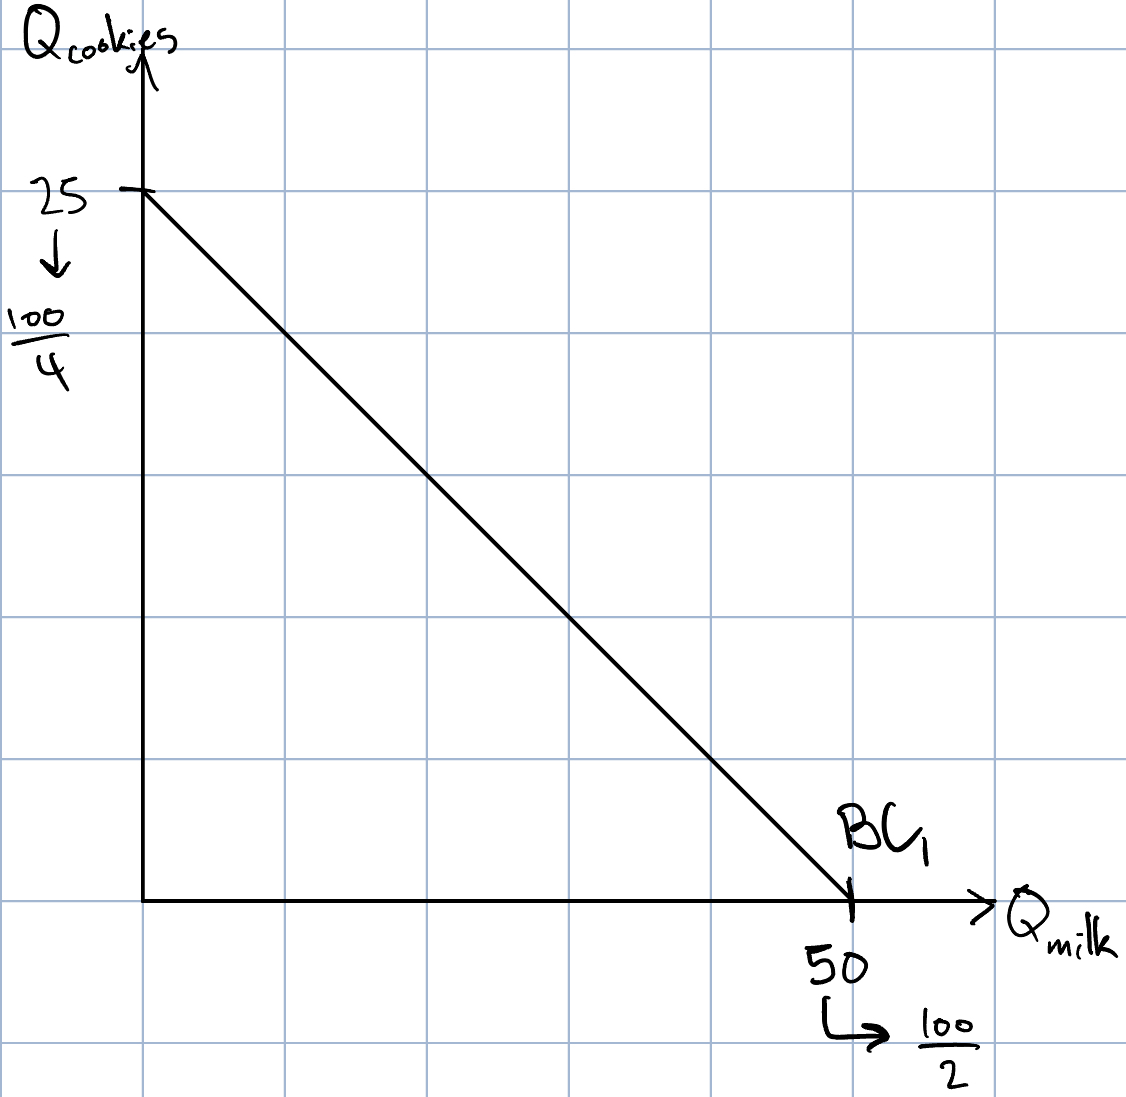
\includegraphics[width = 0.5\textwidth]{2a}
		\end{center}
		
	\newpage
	
	\item His optimal bundle wouldn't change because his budget constraint doesn't change.
	
		\begin{center}
		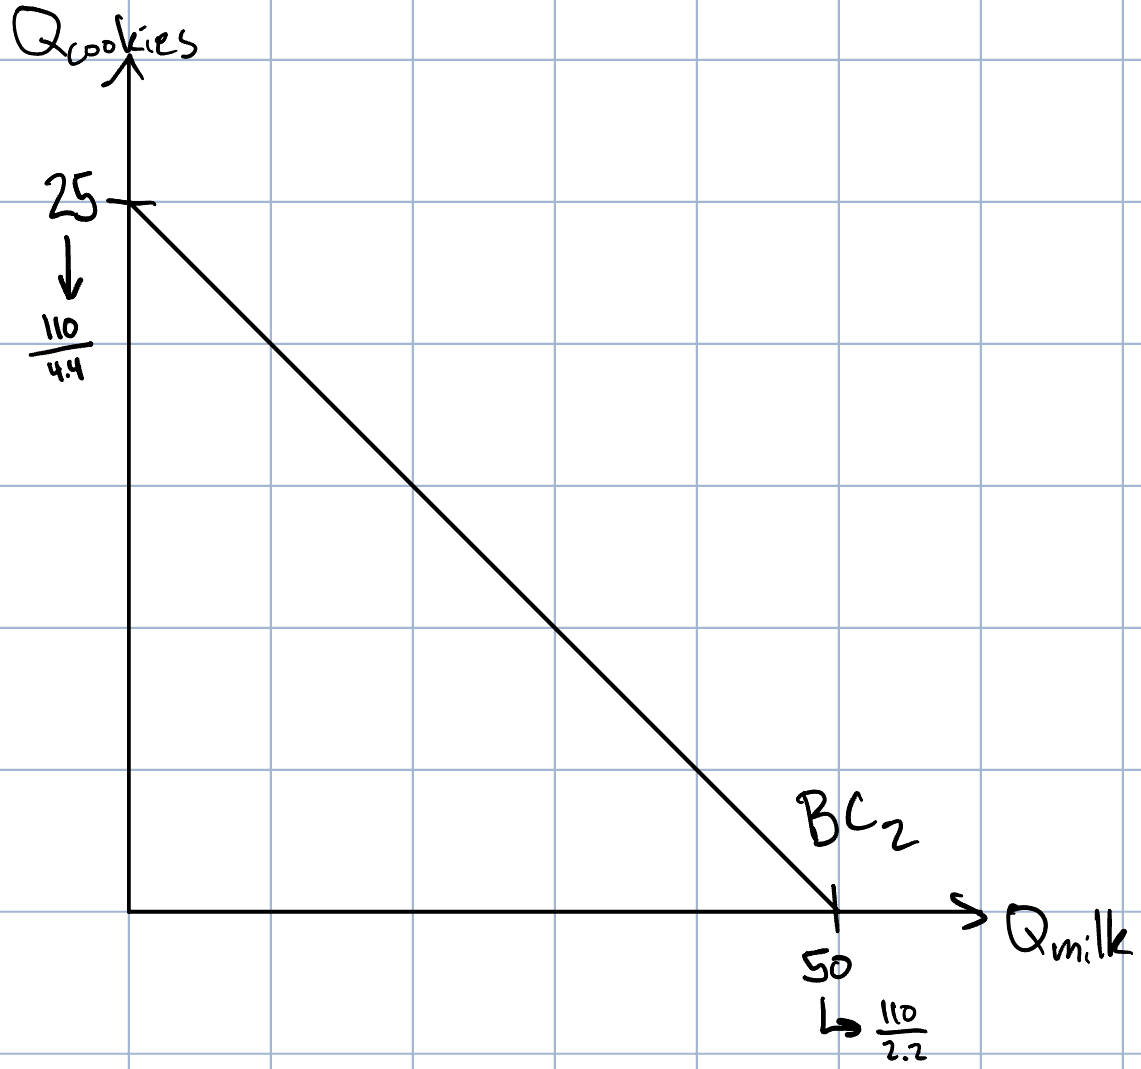
\includegraphics[width = 0.5\textwidth]{2b}
		\end{center}
	
	\end{enumerate}
	
\item If consumers do not buy less of a commodity when their incomes rise, then the commodity is a normal good. When the price of a normal good rises, the substitution effect and the income effect are both negative. The substitution effect is negative because the good becomes relatively more expensive. The income effect is negative because the price increase lowers their purchasing power, and people consume less of a normal good when purchasing power declines. Since both effects are negative, the overall effect of a price increase is that consumers buy less of the commodity.

\item Below, I plot the marginal utility per dollar for each person.

		\begin{center}
		\begin{tabular}{| c | c | c |}
		\hline
		& \makecell{MU/\$ of\\Apples} & \makecell{MU/\$ of\\Pears} \\
		\hline
		Claire & 6 & 6 \\
		\hline
		Phil & 6 & 3 \\
		\hline
		Haley & 6 & 1.5 \\
		\hline
		Alex & 3 & 3 \\
		\hline
		Luke & 3 & 6 \\
		\hline
		\end{tabular}
		\end{center}
		
	Only Claire and Alex are optimizing their choice of fruit because only Claire and Alex have equalized their marginal utility per dollar for apples and pears. Phil and Haley should spend more on apples and less on pears because their marginal utility per dollar is higher for apples. Luke should spend more on pears and less on apples because his marginal utility per dollar is higher for pears.

\item It's possible but not plausible.

When wage goes up, consumption becomes relatively cheaper because it requires less work than it used to in order to afford a certain level of consumption. Since consumption becomes relatively cheaper, the substitution effect is positive.

An increase in wage also increases a person's purchasing power, so they become effectively richer. The only reasonable assumption is that consumption is a normal good. In that case, the income effect is positive.

Since both the income and the substitution effect are positive, the overall effect on consumption is positive. That's to say consumption increases when wage increases.

We could implausibly assume that consumption was a highly inferior good. Then the income effect would be negative. If the income effect were so negative that it outweighed the substitution effect, then the overall effect would be negative, and consumption would decrease. That's tantamount to assuming that consumption is a Giffen good because we're saying demand for consumption decreases when the price of consumption decreases.

\end{enumerate}

\end{document}